\section{Actuation module}

With the \emph{perception} module the system obtains the maximum possible certainty about the persons present in the current RGB image, as well as their condition of being or not being the one to be followed. The \emph{actuation} module is responsible of generating a suitable command to the robot motors, in order to move towards the followed target person, in case it is seen in the current frame. To do so, it follows its own pipeline, explained next.

%\subsection{Following behavior}
% As it has been stated, 
The input for this module is the information yielded by the \emph{perception} module: the \emph{tracked persons} parameters (position, face, ``is or is not the target person"). From this information, it has to infer the proper robot movements taking also into account the state of the system on the last iteration. This is implemented with a \emph{case-based} behavior, which follows the \emph{flow chart} represented on Fig. \ref{fig:actuation_flow}. The response mainly depends on \emph{mom} (the name given to the target person), as it can be \emph{lost} or \emph{tracked and followed}.\\

\begin{figure}[h]
	\centering
	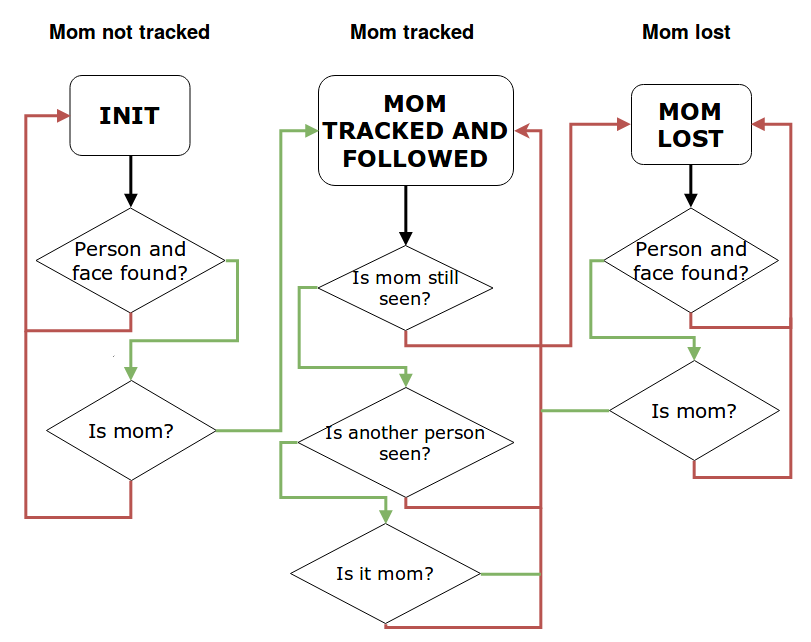
\includegraphics[width=9cm]{images/flowchart}
	\caption{\emph{Flow chart} followed by the case-based behavioral, depending on the previous state.}
	\label{fig:actuation_flow}
\end{figure}

If the target person is found among the tracked persons, the system follows it. It can be observed that the system does not need a continuous face feedback to follow the target person. The time-spatial continuity provided by the previously described trackers allows the person tracking even when only the person back side is visible. In addition, if a new face is found and it satisfies the criteria of similarity with the reference face, then the \emph{followed} role is switched to that new person, which begins to be followed by the robot.

This actuation module has been implemented within a computer iterative thread, and its pipeline is executed \emph{once} per thread iteration. This results on a new speed command pair (angular and linear speeds) to the motor base on each iteration.

\subsection{Error computation}

Once the system has recognized the target person inside the image, in case it is being seen, it proceeds to an \emph{error computation}, in order to determine the strength of the required rotation and traslation to move towards that person. As the robot moves over the ground plane, with two degrees of freedom, the system computes two errors: angular error and distance error.

\begin{figure}
  \centering
  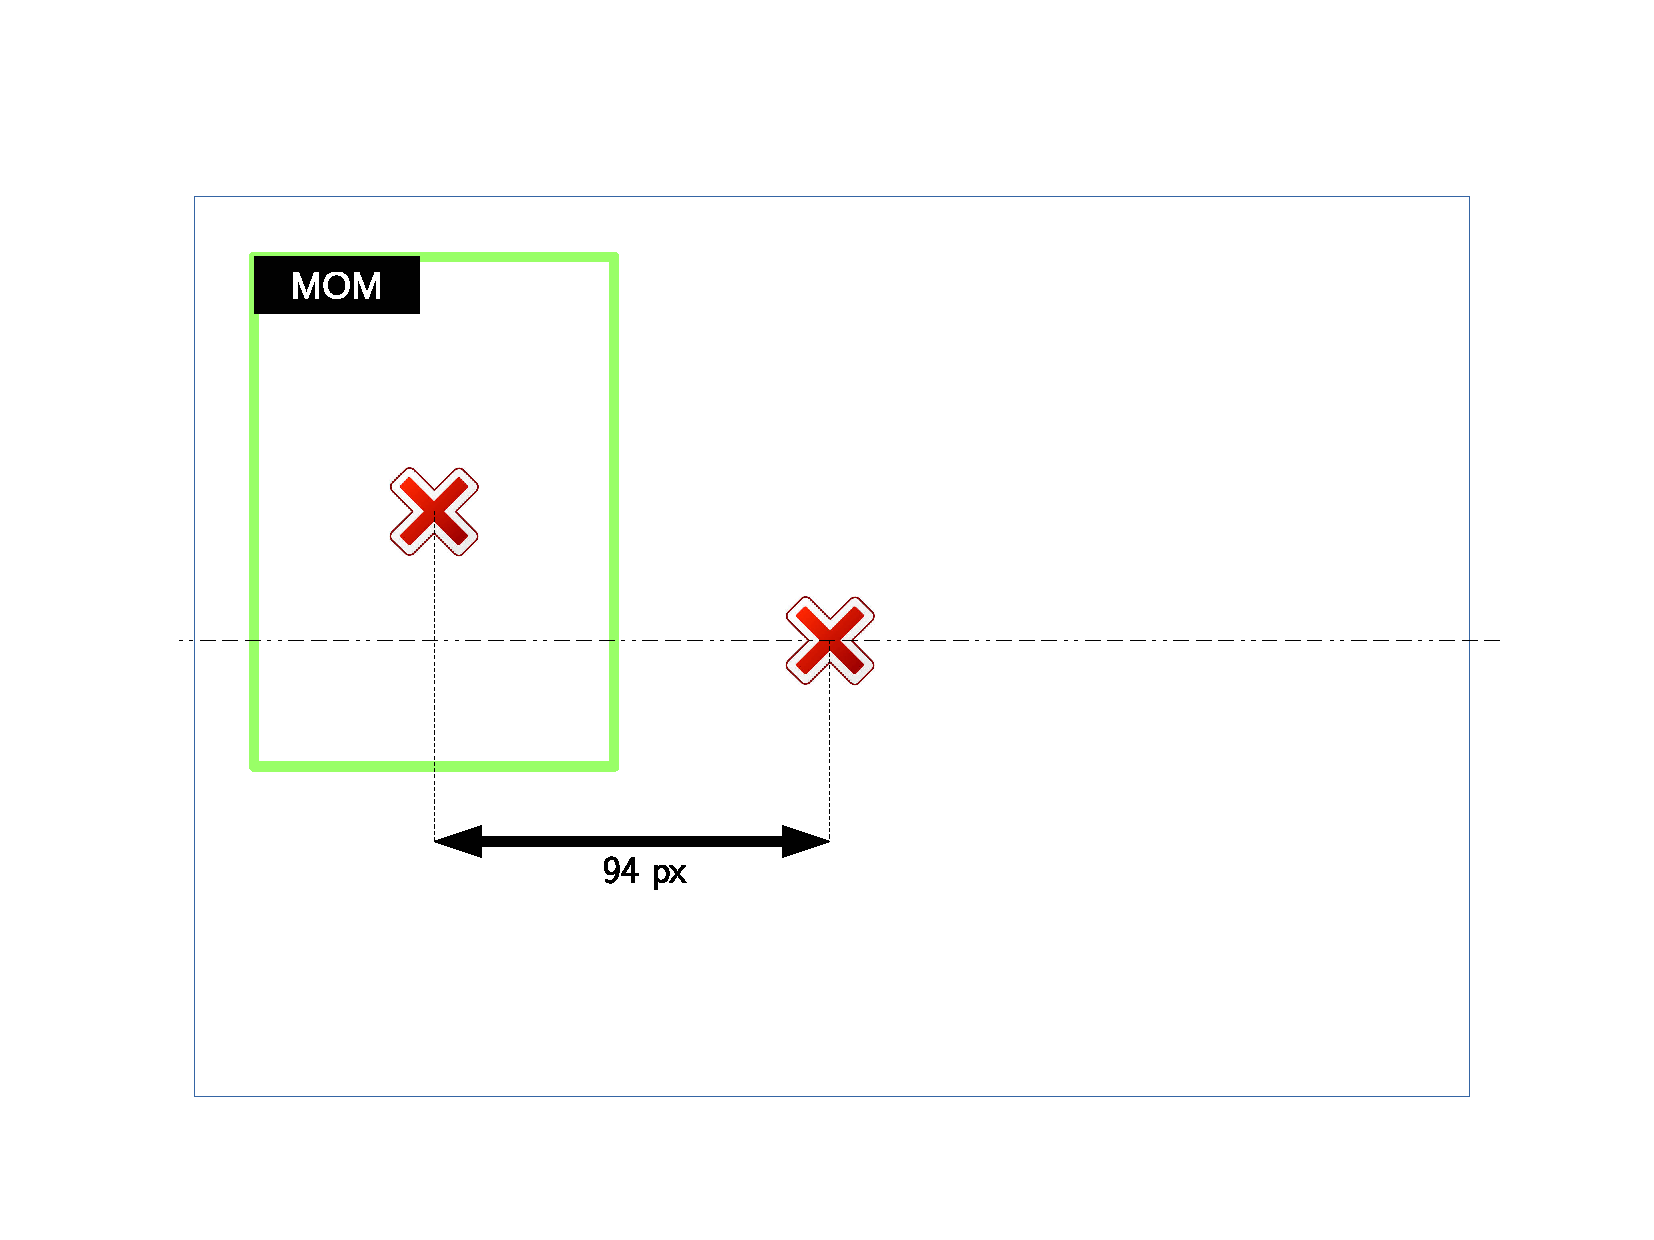
\includegraphics[width=6cm]{images/h_error}
  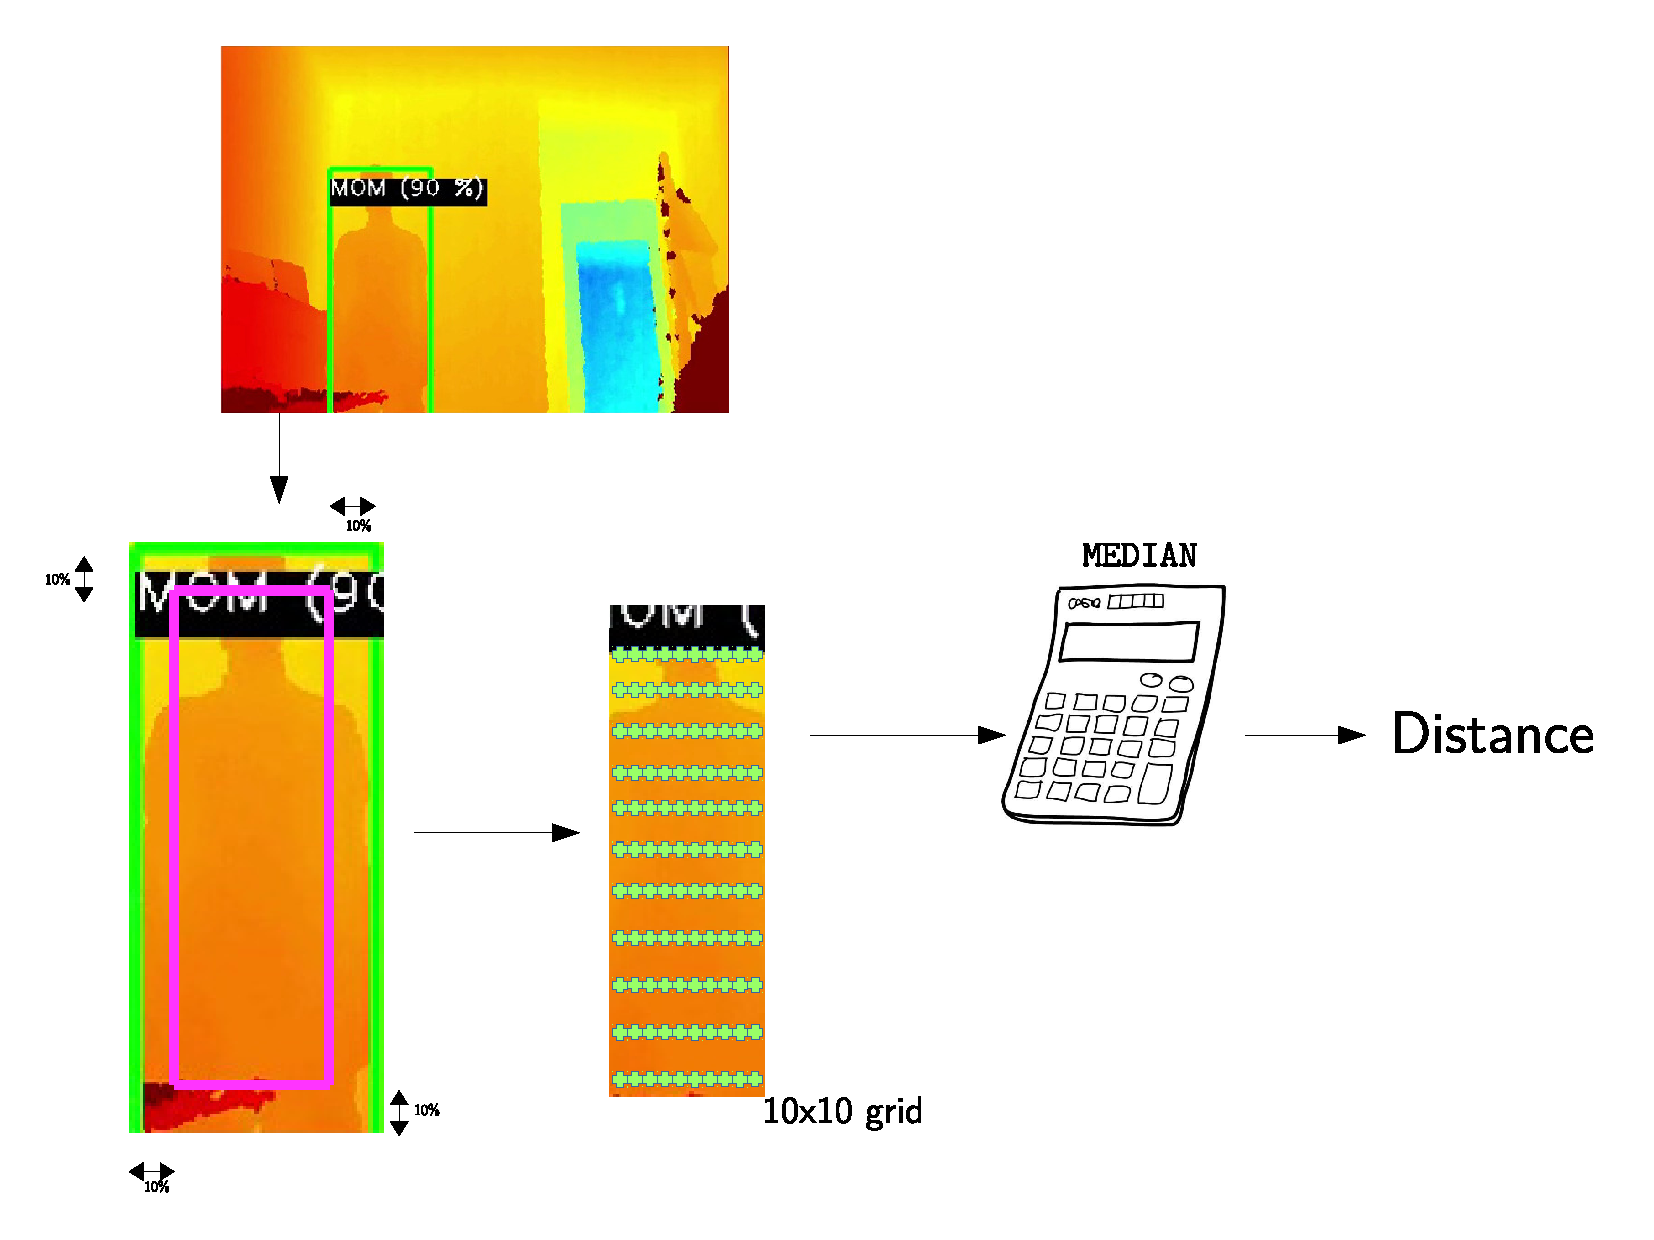
\includegraphics[width=6cm]{images/distance_error}
  \caption{Computation of the angular error (left) and distance error (right) between the system and the followed person.}
  \label{fig:h_error}
\end{figure}

The most desirable robot orientation with respect to the person is to be aligned with her. This way, the person appears right in the horizontal center of the image. Hence, we can compute the \emph{angular error} as the subtract of the center coordinates and the center of the person's bounding box, in the horizontal dimension (Figure \ref{fig:h_error} (left)). This error gives an approximate idea of the necessary turn to align the robot and the target person.
	
The used sensor is a RGBD camera, which provides \emph{depth} images. As it is aligned with the RGB image, the coordinates of the person inside the depth image are the same than the RGB ones. Hence, it allows to \emph{locate} the person inside the depth map and measure the \emph{distance error}. For the sake of robustness, this has been implemented using a 10$\times$10 grid sampling of the depth values inside the person box (putting care on avoiding the margins, in order to measure only inside the person) allows to collect a serie of measured distances to the person. It computes the \emph{median} of that set of measures, taking the result as the real distance from the robot to the person, as seen on Fig. \ref{fig:h_error} (right). 
%So far, the system is capable to determine a numerical error value to measure the magnitude of the required response.

\subsection{Movement control}

Both angular and distance errors are computed to determine the \emph{relative position} of the robot and the target person. They are used as an input to compute the most suitable control response. As the purpose is not to move the robot literally to the position of the person, but to just maintain a following behavior, a \emph{desirable zone} is established in each degree of freedom. When the target person is found inside these desirable zones (illustrated on Fig.\ref{fig:dead_zones}) the robot will not move towards her, as the person is considered \emph{under control}. They are also known as dead zones as no correction from control is needed. 

\begin{figure}[h]
	\centering
	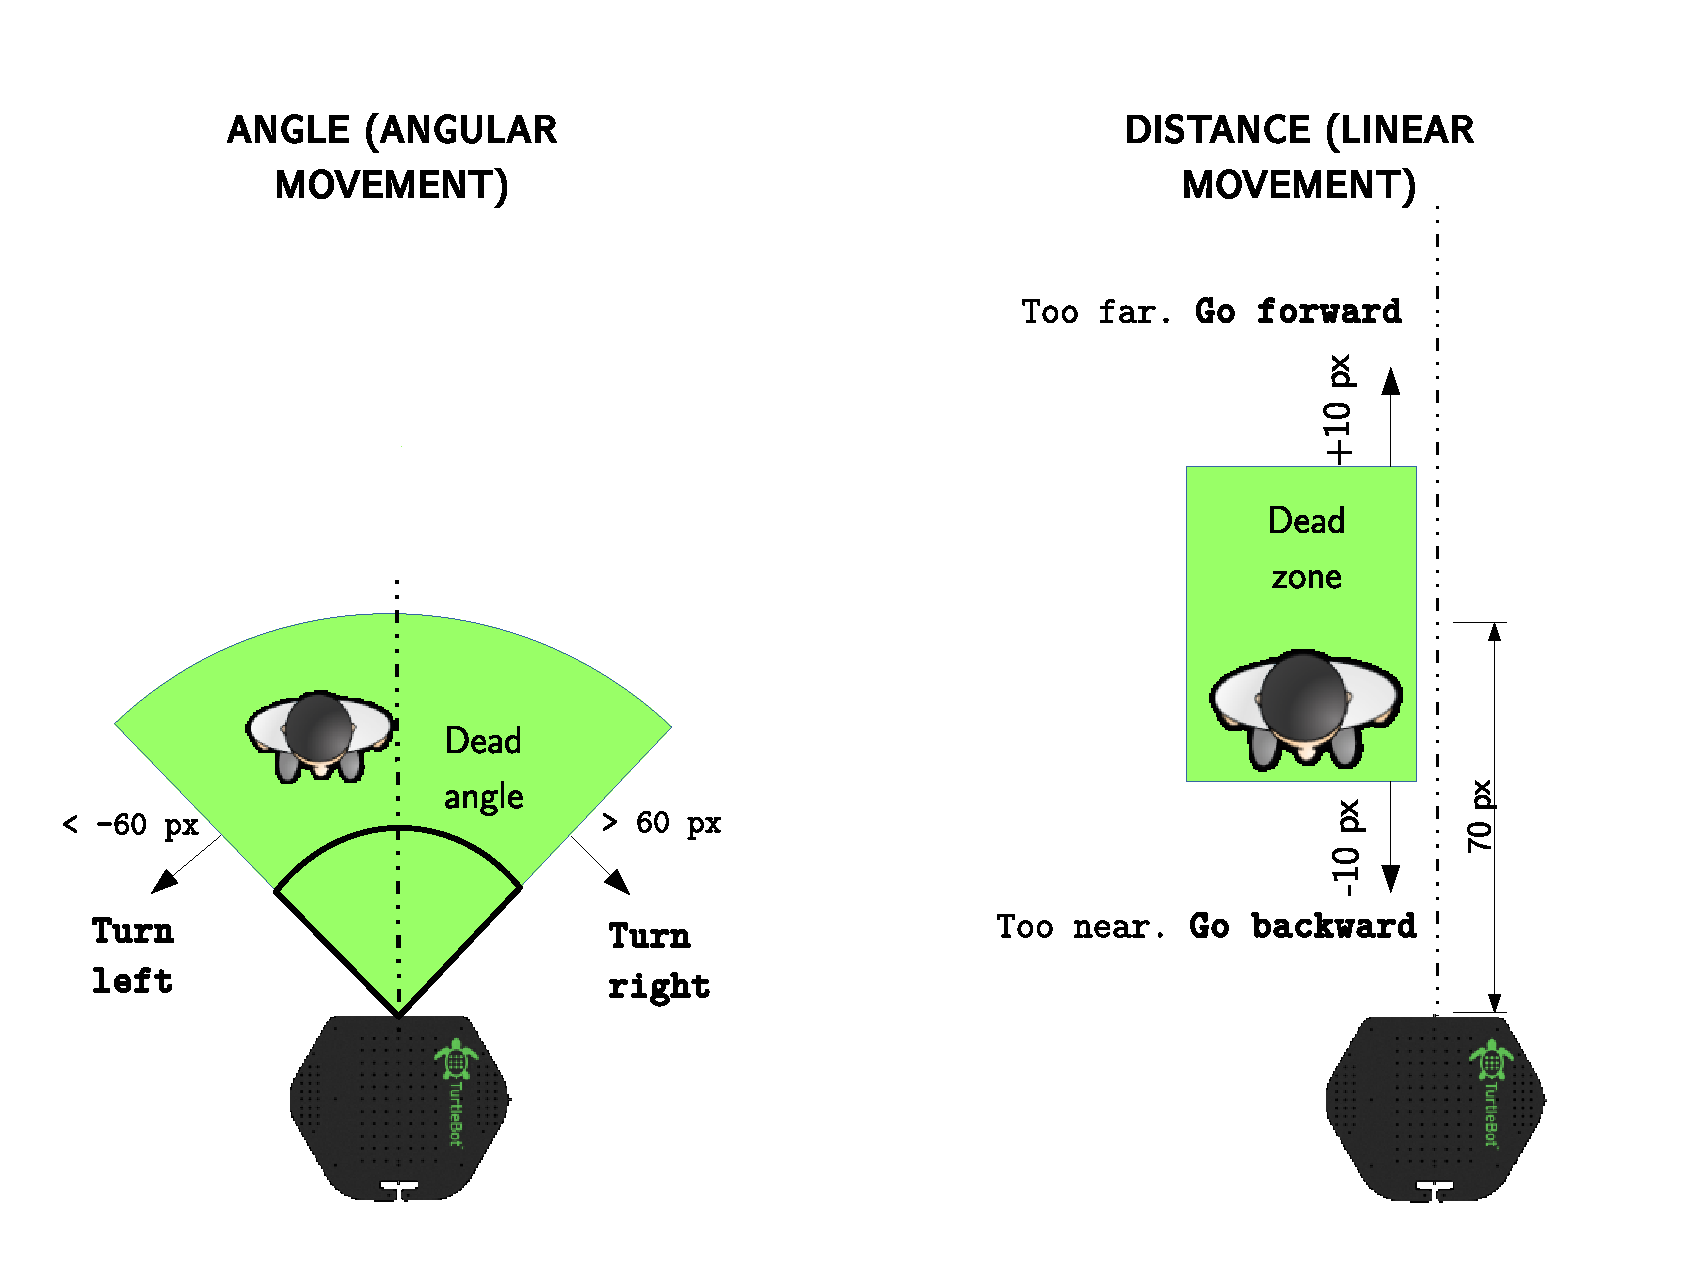
\includegraphics[width=11cm]{images/dead_zones}
	\caption{Dead zones on each dimension, where the person is considered under control.}
	\label{fig:dead_zones}
\end{figure}

If the person is outside these dead zones, a physical correction response is required, with the purpose of \emph{seeing} that person again inside the dead zone. For this action, each dimension implements a \emph{PID} controller, which establishes a \emph{closed-loop} feedback, as described on \cite{pid-controller}. This allows to keep in mind previous responses, to achieve the optimum fitting on each iteration. This means, for example, to accelerate if the person is not going any closer, or to step hard on the brake if the person suddenly gets too close.

The implemented \emph{PID} controllers (an angular and a linear one) have been experimentally tuned to obtain the most suitable parameters for our operation, obtaining the values in Table \ref{tab:pids}.

\begin{table}[h]
	\centering
	\begin{tabular}{|c|c|c|}
		\hline
		\textbf{} & \textbf{Linear} & \textbf{Angular} \\ \hline
		$k_p$     & 2               & 7                \\ \hline
		$k_d$     & 0.1             & 0.5              \\ \hline
		$k_i$     & 3               & 10               \\ \hline
	\end{tabular}
	\caption{Optimal found values for the parameters in each PID controller.}
	\label{tab:pids}
\end{table}

This way, the system can output a speed command with a tight adjustment to the values required by the situation of the current iteration. The response obtained from this value is a \emph{reactive} one. This means that each value results in a new movement command, avoiding to perform movements longer than one iteration. For softness sake, what is sent to the motors is not that value, but the \emph{mean} between it and the last sent one. This way, it results on a slightly longer convergence that helps to remove sudden movements.


